\scanpage{4}
% Faint reversed typescript is show-through from the other face of the sheet.
Multistrates orientés -- \uline{magasins \unsure{orienteurs}}

Données d'un magasin \unsure{orienteur} :
\[
M,\ \underset{\substack{\text{incidence}\\\text{immédiate}}}{\triangleleft},\ \overset{\circ}{\ll},\ |\circ|,\
\underset{\substack{\text{involution}\\\text{ss pt fixe}\\\text{``multistr. orienté opposé''}}}{\inserted{a:}\ X\mapsto X^-},\ M_0^+\deleted{\unsure{\subset M}}
\]

\uline{Magor. 1}\quad a) $\triangleleft$ antiréflexive. Le préordre strict engendré $<$ ($X<Y$ ssi $\exists\ X_0=X\mathrel{\triangleleft}X_1\mathrel{\triangleleft}\cdots\mathrel{\triangleleft}X_{n-1}\mathrel{\triangleleft}X_n\unsure{=|\leq=}Y$) est un ordre strict (pas de chaînes fermées, i.e. on ne peut avoir $X<X$). Il satisfait la condition des chaînes \deleted{\unsure{descendantes}} \inserted{\unsure{de longueur finie}}.

\deleted{tout élément est de dim. finie, et les éléments minimaux \unsure{qu'il majore|qui le majorent} \unsure{ont une certaine} \illegible{3} \unsure{dans lui}}

(en particulier, tout $X\in M$ de dim. finie pour $\leq$).

% margin note written slanted, down the left edge
\margin{\unsure{Ainsi} $\triangleleft$ \unsure{revient} à donner un ordre strict \unsure{vérifiant} la cond. des chaînes descendantes.}

b) $\overset{\circ}{\ll}$ relation d'ordre

c) $|\circ|$ \deleted{symétrique} antiréflexive.

d) $X\mapsto X^-$, involution sans pt fixe.

(e) $M_0^+$ est une partie de $M$.

(\uline{Magor $1'$} $\deleted{\unsure{\Longleftarrow}}$, (a) $X\triangleleft Y\Longrightarrow X^-\triangleleft Y^-$, $\deleted{\unsure{X\triangleleft Y^-}}$

b) $X\overset{\circ}{\ll}Y'\Longrightarrow X^-\overset{\circ}{\ll}Y^-$

c) $X|\circ|Y\Longrightarrow X^-|\circ|Y$.

\deleted{\unsure{d)}}

\margin{NB On peut avoir à la fois $X\triangleleft Y$ et $X\triangleleft Y^-$.}
\figure{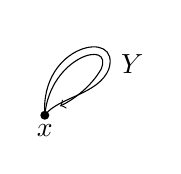
\begin{tikzpicture}[scale=0.65]
\fill (0,0) circle (2.5pt);
\draw (0,0) .. controls (-0.1,1.4) and (1.5,1.7) .. (1.25,0.9) .. controls (1.05,0.4) and (0.25,0.35) .. (0,0);
\draw[->] (0,0) .. controls (0.1,1.15) and (1.35,1.5) .. (1.1,0.9) .. controls (0.9,0.55) and (0.55,0.3) .. (0.3,0.18);
\node[below] at (0,0) {$x$};\node[right] at (1.3,1) {$Y$};
\end{tikzpicture}}

\uline{Magor 2}\quad a) Si $X,Y$ tels que $\exists Y'\quad X\overset{\circ}{\ll}Y'\leq Y$, alors $Y'$ \inserted{\unsure{unique}}

b) Si $X\overset{\circ}{\ll}Y$, et $X'\triangleleft X^{\unsure{\epsilon|\circ}}$, $\exists Y'\triangleleft Y$ avec
\[
X'\overset{\circ}{\ll}Y'
\]

\uline{Magor 3}\quad Si $X|\circ|Y$, et $X'\overset{\circ}{\ll}X$, $Y'\overset{\circ}{\ll}Y$, on a $X'|\circ|Y'$

-- \uline{Magor 4}\quad Si $X<Y$, alors $X|\circ|Y$.

\uline{Magor 6}\quad a) Soient $\unsure{Z|X}<X$, $\operatorname{codim}(\unsure{Y|Z},X)=2$. Alors il n'existe qu'\uline{un seul} $Y^{\unsure{\sharp|*}}$, avec $Z\triangleleft Y^{\sharp}\triangleleft X$, et de plus il existe $Y^{\unsure{\flat|b}}$ avec : $Z^-\triangleleft Y^{\flat}\triangleleft X^{\deleted{\unsure{-}}}$

b) Soit $X$ avec $\dim X=1$. Alors il existe et un seul $x\in M_0^+$, $x\triangleleft X$ \inserted{(i.e. $x\unsure{\in|=}M_0$)}

% A large marginal arrow points from Magor 5 to the space after Magor 4.
\margin{\figure{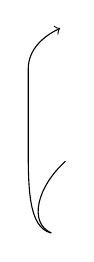
\begin{tikzpicture}[x=0.45cm,y=0.65cm]
\draw[->] (0,-4) .. controls (-0.65,-3.9) and (-0.65,-3.1) .. (-0.65,-2.3) -- (-0.65,-0.8) .. controls (-0.65,-0.4) and (-0.2,-0.15) .. (0.25,0);
\draw (0,-4) .. controls (-0.65,-3.8) and (-0.4,-3.1) .. (0.4,-2.6);
\end{tikzpicture}}}
\uline{Magor 5}\quad a) $x\in M_0^+\Longrightarrow\dim x=0$, i.e. $\overline{\exists}\ y$ avec $y\triangleleft x$.

b) On a $M_0=M_0^+\amalg a(M_0^+)$, i.e. \deleted{\unsure{x}} $x\in M_0^+\Longrightarrow x^-\notin M_0^+$, et $\forall x\in M_0$, on a $x\in M_0^+$ ou $x^-\in M_0^+$.
% archive sheet number: 3
